\chapter{Specifikacija programske potpore}
		
	\section{Funkcionalni zahtjevi}
			
			
			\noindent \textbf{Dionici:}
			
			\begin{packed_enum}

				 \item Korisnici treninga
				 \item Treneri
			     \item Administrator
			     \item Neregistrirani korisnici

				
			\end{packed_enum}
			
			\noindent \textbf{Aktori i njihovi funkcionalni zahtjevi:}
			
			
			\begin{packed_enum}


				\item  \underbar{Neregistrirani/neprijavljeni korisnik (inicijator) može:}
				
				\begin{packed_enum}
					
					\item registrirati se
					\item gumbom izbrisati sve unesene podatke pri registraciji
					\item prijaviti se
					\item pregledati početnu stranicu aplkacije
										
				\end{packed_enum}
			
				\item  \underbar{Korisnik treninga (inicijator) može:}
				
				\begin{packed_enum}
					
					\item prijaviti se u sustav korisničkim imenom i lozinkom
					\item pregledavati i mijenjati svoje osobne podatke (lozinku)
					\item vidjeti kroz kalendar kojim treninzima može prisustvovati ovisno o vježbama koje mora odrađivati
					\item rezervirati treninge na koje želi ići ovisno o fondu sati kojeg ima
					\item otkazati rezervaciju treninga
					
				\end{packed_enum}
			
			    \item  \underbar{Trener (inicijator) može:}
			    
			    \begin{packed_enum}
			    	
			    	\item prijaviti se u sustav koristeći ime i lozinku
			    	\item pregledavati sve registrirane korisničke račune
			    	\item odabrati registriranog korisnika treninga kojem može dodijeliti vježbe ovisno o ciljevima osobe
			    	\item stvarati treninge na mjesečnoj bazi (definirati vježbe i maksimalan broj polaznika) te ih unositi u kalendar
 			    	\item upisuje pravila o rezervaciji
			    	
			    \end{packed_enum}
		       
		        \item  \underbar{Administrator (inicijator) može:}
		        
		        \begin{packed_enum}
		        	
		        	\item prijaviti se
		        	\item administrirati korisničke račune te račune trenera
		        	\item ažurirati sve podatke u aplikaciji
		        	\item registrirati trenere
		        	
		        \end{packed_enum}

			\end{packed_enum}
			
			\eject 
			
			
				
			\subsection{Obrasci uporabe}
				
				
				\subsubsection{Opis obrazaca uporabe}
					

					\noindent \underbar{\textbf {UC1-Registracija}}				\begin{packed_item}
	
						\item \textbf{Glavni sudionik: }Neregistrirani korisnik treninga
						\item  \textbf{Cilj:} Stvoriti korisnički račun
						\item  \textbf{Sudionici:} Baza podataka
						\item  \textbf{Preduvjet:} UC15
						\item  \textbf{Opis osnovnog tijeka:}
						
						 \begin{packed_enum}
                      
	                        \item Neregistrirani korisnik odabire akciju "Registration" na početnoj stranici
	                        \item Sustav otvara formu za upis podataka
							\item Neregistrirani korisnik upisuje potrebne podatke (ime, prezime, koriničko ime, email, lozinku i ciljeve)
							\item Neregistrirani korisnik odabire opciju "Submit" 
							\item Sustav provjerava ispravnost unesenih podataka, sprema ih u bazu, prijavljuje korisnika, postavlja vrijeme isteka sesije na 30 minuta i otvara stranicu s osobnim podacima
							
						
						\end{packed_enum}
						
						\item*  \textbf{Opis mogućih odstupanja:}
						cx 5 m+cij9 jij66 +
						 \begin{packed_enum}
						 	\item[4.a] Neregistrirani korisnik odabire akciju Reset, a sustav na formi registracije briše sve unesene podatke. Sustav nastavlja izvođenje scenarija u koraku 3.
							\item[5.a] Sustav provjerava i utvrđuje da uneseni podaci nisu ispravni. Obavještava korisnika odgovarajućom porukom te nastavlja izvođenje scenarija u koraku 3 
							

								
						  \end{packed_enum}
						
					\end{packed_item}
				
				\noindent \underbar{\textbf {UC2-Prijava}}				\begin{packed_item}
						
						\item \textbf{Glavni sudionik: }Korisnik treninga, trener, administrator
						\item  \textbf{Cilj:} Prijaviti se u aplikaciju
						\item  \textbf{Sudionici:} Baza podataka
						\item  \textbf{Preduvjet:} UC15
						\item  \textbf{Opis osnovnog tijeka:}
						
						\item \begin{packed_enum}

							\item  Neprijavljeni korisnik odabire akciju "Log in" na početnoj stranici
							\item Sustav otvara formu za upis podataka
							\item Neprijavljeni korisnik upisuje potrebne podatke u formu (korisničko ime i lozinku)
							\item Sustav provjerava ispravnost podataka, prijavljuje korisnika, postavlja vrijeme isteka sesije na 30 minuta i otvara stranicu s osobnim podacima

							
						\end{packed_enum}
						
						\item  \textbf{Opis mogućih odstupanja:}
						
						\begin{packed_enum}
							
							\item[1.a] Ako neprijavljeni korisnik nema račun može izabrati akciju "Nemaš račun?" te sustav otvara formu za Registraciju
							\item[3.a] Sustav provjerava i utvrđuje da uneseni podaci nisu ispravni. Obavještava korisnika odgovarajućom porukom te nastavlja izvođenje scenarija u koraku 2
							
						\end{packed_enum}
						
					\end{packed_item}
				   
				\noindent \underbar{\textbf {UC3-Pregled osobnih podataka}}	\begin{packed_item}
						
						\item \textbf{Glavni sudionik: }Korisnik treninga, trener, administrator

						\item  \textbf{Cilj:} Pregled osobnih podataka

						\item  \textbf{Sudionici:} Baza podataka
						\item  \textbf{Preduvjet:} UC2
						\item  \textbf{Opis osnovnog tijeka:}
						
						\item[] \begin{packed_enum}
							
							\item Sustav prijavljenog korisnik nakon prijave/registracije automatski odvodi na stranicu osobnih podataka ili prijavljeni korisnik odabire akciju "Moji podaci" u zaglavlju aplikacije
							\item Korisnik ima uvid u svoje podatke (ime, prezime, koriničko ime, email, avatar)

							
						\end{packed_enum}
						
						\item  \textbf{Opis mogućih odstupanja:}
						
						\begin{packed_enum}
							
							\item /
							
						\end{packed_enum}
						
					\end{packed_item}
				
				\noindent \underbar{\textbf {UC4-Promjena osobnih podataka}}				\begin{packed_item}
						
						\item \textbf{Glavni sudionik: }Korisnik treninga
						\item  \textbf{Cilj:} Promjena svojih osobnih podataka
						\item  \textbf{Sudionici:} Baza podataka
						\item  \textbf{Preduvjet:} UC3
						\item  \textbf{Opis osnovnog tijeka:}
						
						\item[] \begin{packed_enum}

							
							\item Korisnik odabire akciju "Izmijeni"
							\item Sustav otvara formu za izmjenu lozinke
							\item Korisnik Nakon promjene odabire akciju "Save changes" 
							\item Sustav provjerava ispravnost podataka, sprema nove podatke u bazu i otvara stranicu s osobnim podacima

							
						\end{packed_enum}
						
						\item  \textbf{Opis mogućih odstupanja:}
						
						\begin{packed_enum}
							
							\item[4.a] Ako je korisnik mijenjao lozinku, sustav provjerava i utvrđuje da unesena stara lozinka nije ispravna. Obavještava korisnika odgovarajućom porukom te nastavlja izvođenje scenarija u koraku 2
							
						\end{packed_enum}
						
					\end{packed_item}
				
				
				\noindent \underbar{\textbf {UC5-Odabir ciljeva}}				\begin{packed_item}
						
						\item \textbf{Glavni sudionik: }Korisnik treninga
						\item  \textbf{Cilj:} Odabir ciljeva za taj mjesec
						\item  \textbf{Sudionici:} Baza podataka, trener
						\item  \textbf{Preduvjet:} UC3  
						\item  \textbf{Opis osnovnog tijeka:}
						
						\item[] \begin{packed_enum}

							\item Korisnik na stranici osobnih podataka iz padajućih izbornika odabire ciljeve
							\item Korisnik odabire akciju "Promijeni ciljeve"
							\item Sustav provjerava ima li korisnik pravo na promjenu ciljeva, mijenja ciljeve u bazi i otvara ponovno stranicu osobnih podataka

							
						\end{packed_enum}
						
						\item  \textbf{Opis mogućih odstupanja:}
						
						\begin{packed_enum}
							
							\item[1.a] Sustav je pri prijavi utvrdio da je korisnik taj mjesec već promijenio ciljeve i onemogućuje padajuće izbornike i gumb "Promijeni ciljeve".
							
						\end{packed_enum}
						
					\end{packed_item}
				
					\noindent \underbar{\textbf {UC6-Pregled termina treninga}}		
						\begin{packed_item}
						
						
						\item \textbf{Glavni sudionik: }Korisnik treninga
						\item  \textbf{Cilj:} Pregled datuma treninga
						\item  \textbf{Sudionici:} Baza podataka
						\item  \textbf{Preduvjet:} UC2
						\item  \textbf{Opis osnovnog tijeka:}
						
						\item[] \begin{packed_enum}
							
							\item Korisnik odabire akciju "Rezervacije" u zaglavlju aplikacije 
							\item Sustav otvara kalendar s terminima treninga koje taj korisnik može rezervirati i naznačenim preostalim satima
							\item Korisnik odabire jedan od dostupnih treninga 
							\item Susatv prikazuje u popup prozoru detalje o terminu (vrijeme početka, vrijeme kraja, ime i prezime trenera, listu vježbi i broj preostalih mjesta)

							
						\end{packed_enum}
						
						\item  \textbf{Opis mogućih odstupanja:}
						
						\begin{packed_enum}
							
							\item[3.a] Sustav utvrđuje da korisniku nisu dodijeljene vježbe pa time ni treninzi te obavještava korisnika porukom na sredini ekrana.
							
						\end{packed_enum}
						
					\end{packed_item}
				
				
					\noindent \underbar{\textbf {UC7-Rezervacija termina treninga}}		
						\begin{packed_item}
						
						\item \textbf{Glavni sudionik: }Korisnik treninga
						\item  \textbf{Cilj:}Rezervacija termina
						\item  \textbf{Sudionici:} Baza podataka
						\item  \textbf{Preduvjet:} UC6
						\item  \textbf{Opis osnovnog tijeka:}
						
						\item[] \begin{packed_enum}

							\item Korisnik nakon odabira treninga odabire akciju "Reserve" 
							\item Sustav provjerava fond sati, smanjuje ih za 1, sprema podatke za korisnika i termin u bazu te otvara stranicu Rezervacije
							\item Sustav rezrviranom treningu nadodaje akciju "Cancel reservation"

							
						\end{packed_enum}
						
						\item  \textbf{Opis mogućih odstupanja:}
						
						\begin{packed_enum}
							
							\item[1.a] Sustav utvrđuje da u terminu nema više slobodnih mjesta te onemogućuje gumb Reserve za taj termin
							\item[1.b] Sustav utvrđuje da korisnik nema više preostalih sati, onemogućuje gumb Reserve i obavještava korisnika porukom iznad kalendara
							
						\end{packed_enum}
						
					\end{packed_item}
				
				
					\noindent \underbar{\textbf {UC8-Pregled datuma treninga i termina po danu 2}}				\begin{packed_item}
						
						\item \textbf{Glavni sudionik: }Trener
						\item  \textbf{Cilj:} Pregled datuma treninga 
						\item  \textbf{Sudionici:} Baza podataka
						\item  \textbf{Preduvjet:} UC2
						\item  \textbf{Opis osnovnog tijeka:}
						
						\item[] \begin{packed_enum}
							
							\item Trener odabire akciju "Termini" u zaglavlju aplikacije 
							\item Sustav otvara kalendar sa svim terminima drugih trenera i njegovim, posebno obojanim, terminima treninga.
							\item Trener odabire jedan od termina 
							\item Susatv prikazuje u popup prozoru detalje o terminu (vrijeme početka, vrijeme kraja, ime i prezime trenera, listu vježbi i broj preostalih mjesta)

							
						\end{packed_enum}
						
						\item  \textbf{Opis mogućih odstupanja:}
						
						\begin{packed_enum}
							
							\item /
							
						\end{packed_enum}
						
					\end{packed_item}
				
					\noindent \underbar{\textbf {UC9-Unos treninga}}			\begin{packed_item}
						
						\item \textbf{Glavni sudionik: }Trener
						\item  \textbf{Cilj:} Unos novog termina
						\item  \textbf{Sudionici:} Baza podataka
						\item  \textbf{Preduvjet:} UC2
						\item  \textbf{Opis osnovnog tijeka:}
						
						\item[] \begin{packed_enum}
							
							\item Trener odabire akciju "Termini" u zaglavlju aplikacije 
							\item Sustav otvara kalendar sa svim terminima drugih trenera i njegovim, posebno obojanim, terminima treninga.
							\item Trener odabire akciju dodaj termin
							\item Sustav otvara formu za unos podataka
							\item Trener unosi podatke (vrijeme početka treninga, vrijeme kraja, vrstu treninga i broj mjesta) i odabire akciju "Create"
							\item Sustav provjerava unesene podatke, sprema ih u bazu i otvara kalendar s terminima
							
							
						\end{packed_enum}
						
						\item  \textbf{Opis mogućih odstupanja:}
						
						\begin{packed_enum}
							
							\item[6.a] Sustav utvrđuje da postoji preklapanje između tog termina i već postojećeg ili da je prevelik broj polaznika te obavjestava korisnika odgovarajućom porukom i anstavlja izvodenje od koraka 4
							
						\end{packed_enum}
						
					\end{packed_item}
					
					
				   	\noindent \underbar{\textbf {UC10-Pregled liste registriranih korisnika}}
				   		
				   				
				   		\begin{packed_item}
				   		
				   		\item \textbf{Glavni sudionik: }Trener
				   		\item  \textbf{Cilj:}Pregled korisnika treninga
				   		\item  \textbf{Sudionici:} Baza podataka
				   		\item  \textbf{Preduvjet:} UC2
				   		\item  \textbf{Opis osnovnog tijeka:}
				   		
				   		\item[] \begin{packed_enum}
				   			
				   			\item Trener odabire akciju "Korisnici" u zaglavlju aplikacije
				   			\item Sustav otvara stranicu s listom registriranih korisnika treninga, oni bez dodijeljenih vježbi su obojani drugačije i imaju uz sebe gumb "Dodijeli vježbu"
				   			
				   		\end{packed_enum}
				   		
				   		\item  \textbf{Opis mogućih odstupanja:}
				   		
				   		\begin{packed_enum}
				   			
				   			\item[2.a]Sustav utvrđuje da nema registriranih korisnika te obavještava trenera odgovarajućom porukom
				   			
				   		\end{packed_enum}
				   		
				   	\end{packed_item}
			   	
			   	\noindent \underbar{\textbf {UC11-Dodjela vježbi}}	
			   		
			   		
			   		\begin{packed_item}
			   			
			   			\item \textbf{Glavni sudionik: }Trener
			   			\item  \textbf{Cilj:}Dodjela vježbi korisniku treninga shodno njihovom cilju
			   			\item  \textbf{Sudionici:} Baza podataka, usluga e-pošte
			   			\item  \textbf{Preduvjet:} UC10
			   			\item  \textbf{Opis osnovnog tijeka:}
			   			
			   			\item[] \begin{packed_enum}
			   				
			   				\item Trener odabire akciju "Dodijeli vježbe"
			   				\item Sustav otvara popup prozor s opisom ciljeva tog korisnika i 3 padajuća izbornika za 3 vježbe
			   				\item Trener bira vježbe i odabire akciju "Save"
			   				\item Sustav provjerava vježbe, sprema ih u bazu i otvara nanovo popis korisnika
			   				
			   				
			   			\end{packed_enum}
			   			
			   			\item  \textbf{Opis mogućih odstupanja:}
			   			
			   			\begin{packed_enum}
			   				
			   				\item[4.a] Sustav utvrđuje da je trener odabrao više istih vježbi, obavještava ga porukom i nastavlja od koraka 2
			   				
			   			\end{packed_enum}
			   			
			   		\end{packed_item}
		   		
		   			\noindent \underbar{\textbf {UC12-Brisanje termina treninga 3}}
		   			
		   			
		   			\begin{packed_item}
		   				
		   				\item \textbf{Glavni sudionik: }Administrator
		   				\item  \textbf{Cilj:} Pregled termina
		   				\item  \textbf{Sudionici:} Baza podataka
		   				\item  \textbf{Preduvjet:} UC2
		   				\item  \textbf{Opis osnovnog tijeka:}
		   				
		   				\item[] \begin{packed_enum}
		   					
		   					\item Administrator odabire akciju "Termini" u zaglavlju aplikacije
		   					\item Sustav otvara stranicu s kalendarom sa svim postojećim terminima treninga
		   					\item Administrator odabire termin te odabire opciju "Delete"
		   					\item Sustav briše termin iz baze podataka i otvara nanovo kalendar s terminima
		   					
		   				\end{packed_enum}
		   				
		   				\item  \textbf{Opis mogućih odstupanja:}
		   				
		   				\begin{packed_enum}
		   					
		   					\item /
		   					
		   				\end{packed_enum}
		   				
		   			\end{packed_item}
	   			
	   			
	   				\noindent \underbar{\textbf {UC13-Registracija trenera}}
	   				
	   				
	   				\begin{packed_item}
	   					
	   					\item \textbf{Glavni sudionik: }Administrator
	   					\item  \textbf{Cilj:} Registracija trenera
	   					\item  \textbf{Sudionici:} Baza podataka
	   					\item  \textbf{Preduvjet:} UC2
	   					\item  \textbf{Opis osnovnog tijeka:}
	   					
	   					\item[] \begin{packed_enum}
	   						
	   						\item Administrator odabire akciju "Register Trainer" u zaglavlju aplikacije
	   						\item Sustav otvara formom za upis podataka o novom treneru (ime, prezime, korisničko ime, lozinka, email)
	   						\item Administrator upisuje podatke i odabire akciju "Register"
	   						\item Sustav provjerava podatke sprema trenera u bazu i otvara početnu stranicu
	   						
	   						
	   					\end{packed_enum}
	   					
	   					\item  \textbf{Opis mogućih odstupanja:}
	   					
	   					\begin{packed_enum}
	   						
	   						\item[4.a] Sustav utvrđuje da su uneseni krivi podaci(npr. korisničko ime već postoji), obavještava administratora odgovarajućom porukom i nastavlja od koraka 2
	   						
	   					\end{packed_enum}
	   					
	   				\end{packed_item}
   				
   				\noindent \underbar{\textbf {UC14-Odjava}}
   				
   				
   				\begin{packed_item}
   					
   					\item \textbf{Glavni sudionik: }Prijavljeni korisnik
   					\item  \textbf{Cilj:}Odjava s računa 
   					\item  \textbf{Sudionici:} Baza podataka
   					\item  \textbf{Preduvjet:} UC3
   					\item  \textbf{Opis osnovnog tijeka:}
   					
   					\item[] \begin{packed_enum}
   						
   						\item Korisnik odabire akciju "Log out" 
   						\item Sustav odjavljuje korisnika i otvara početnu stranicu
   						
   						
   					\end{packed_enum}
   					
   					\item  \textbf{Opis mogućih odstupanja:}
   					
   					\begin{packed_enum}
   						
   						\item /
   						
   					\end{packed_enum}
   					
   				\end{packed_item}
   			
   			    \noindent \underbar{\textbf {UC15-Pregled početne stranice}}
   			    
   			    
   			    \begin{packed_item}
   			    	
   			    	\item \textbf{Glavni sudionik: }Korisnik (bilo tko)
   			    	\item  \textbf{Cilj:}Pregled početne stranice aplikacije na kojoj pobliže opisujemo te reklamiramo našu aplikaciju koja koristi za upravljanje grupnih treninga 
   			    	\item  \textbf{Sudionici:} /
   			    	\item  \textbf{Preduvjet:} /
   			    	\item  \textbf{Opis osnovnog tijeka:}
   			    	
   			    	\item[] \begin{packed_enum}
   			    		
   			    		\item Upis adrese naše aplikacije u internet tražilicu
   			    		
   			    	\end{packed_enum}
   			    	
   			    	\item  \textbf{Opis mogućih odstupanja:}
   			    	
   			    	\begin{packed_enum}
   			    		
   			    		\item /
   			    		
   			    	\end{packed_enum}
   			    	
   			    \end{packed_item}
				\subsubsection{Dijagrami obrazaca uporabe}
					
						\begin{figure}[H]
						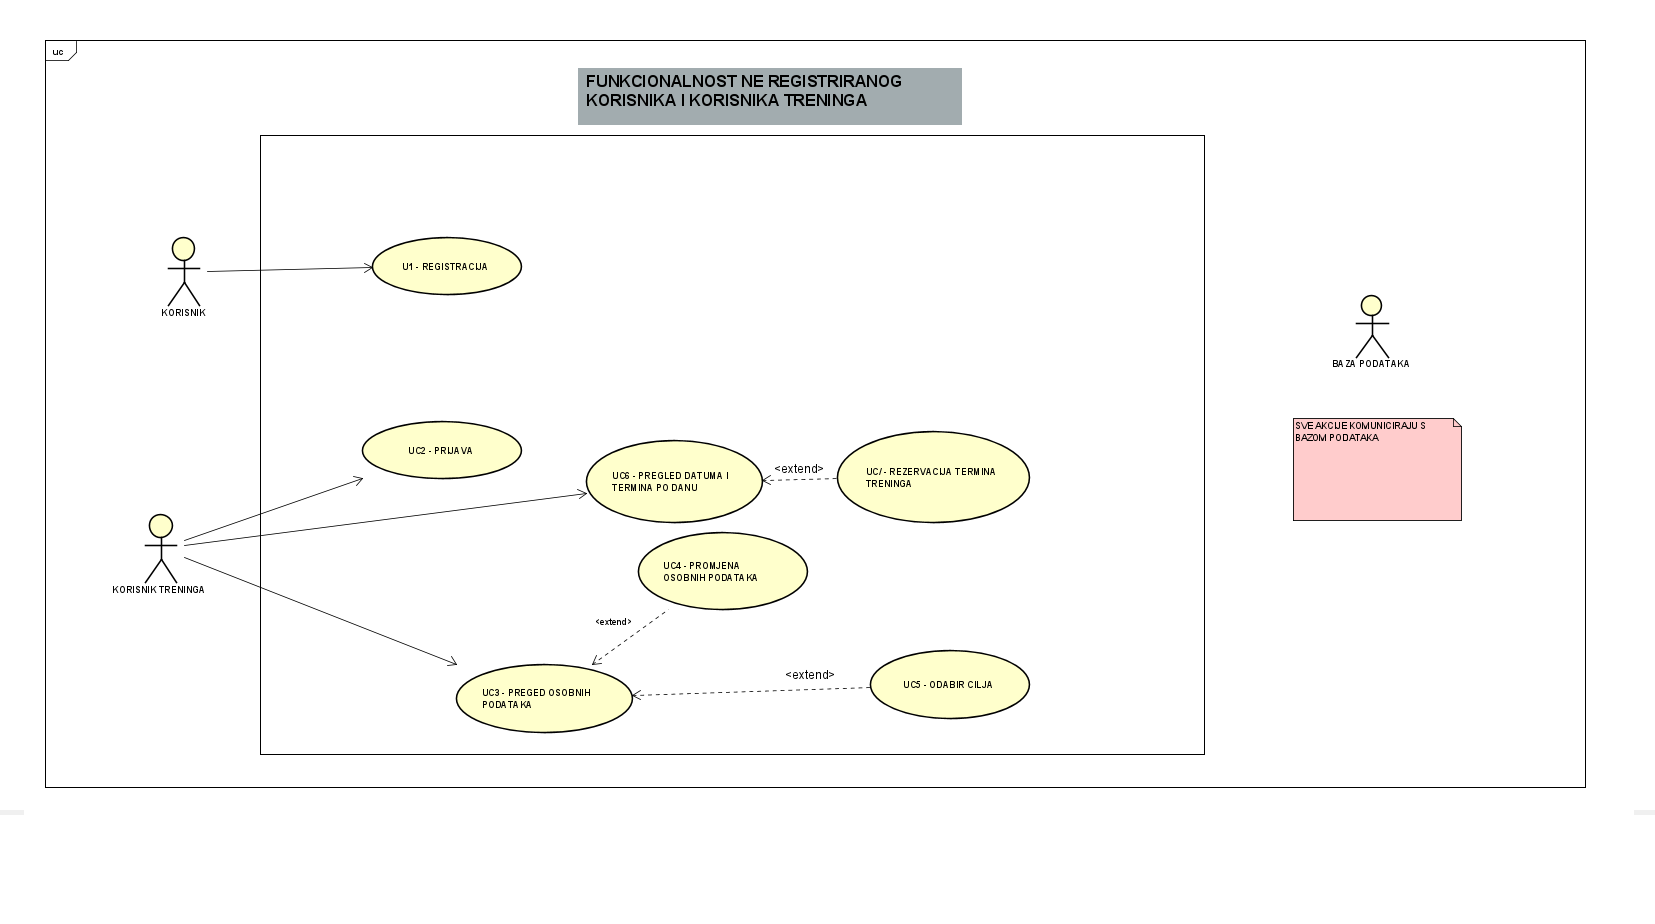
\includegraphics[scale=0.5]{dijagrami/nestodrugo.png} %veličina slike u odnosu na originalnu datoteku i pozicija slike
						\centering
						\caption{"Dijagram funckionalnosti neregistriranog korisnika i korisnika treninga"}
						\label{fig:ou1}
				     	\end{figure}
			     	
			     	\begin{figure}[H]
			     		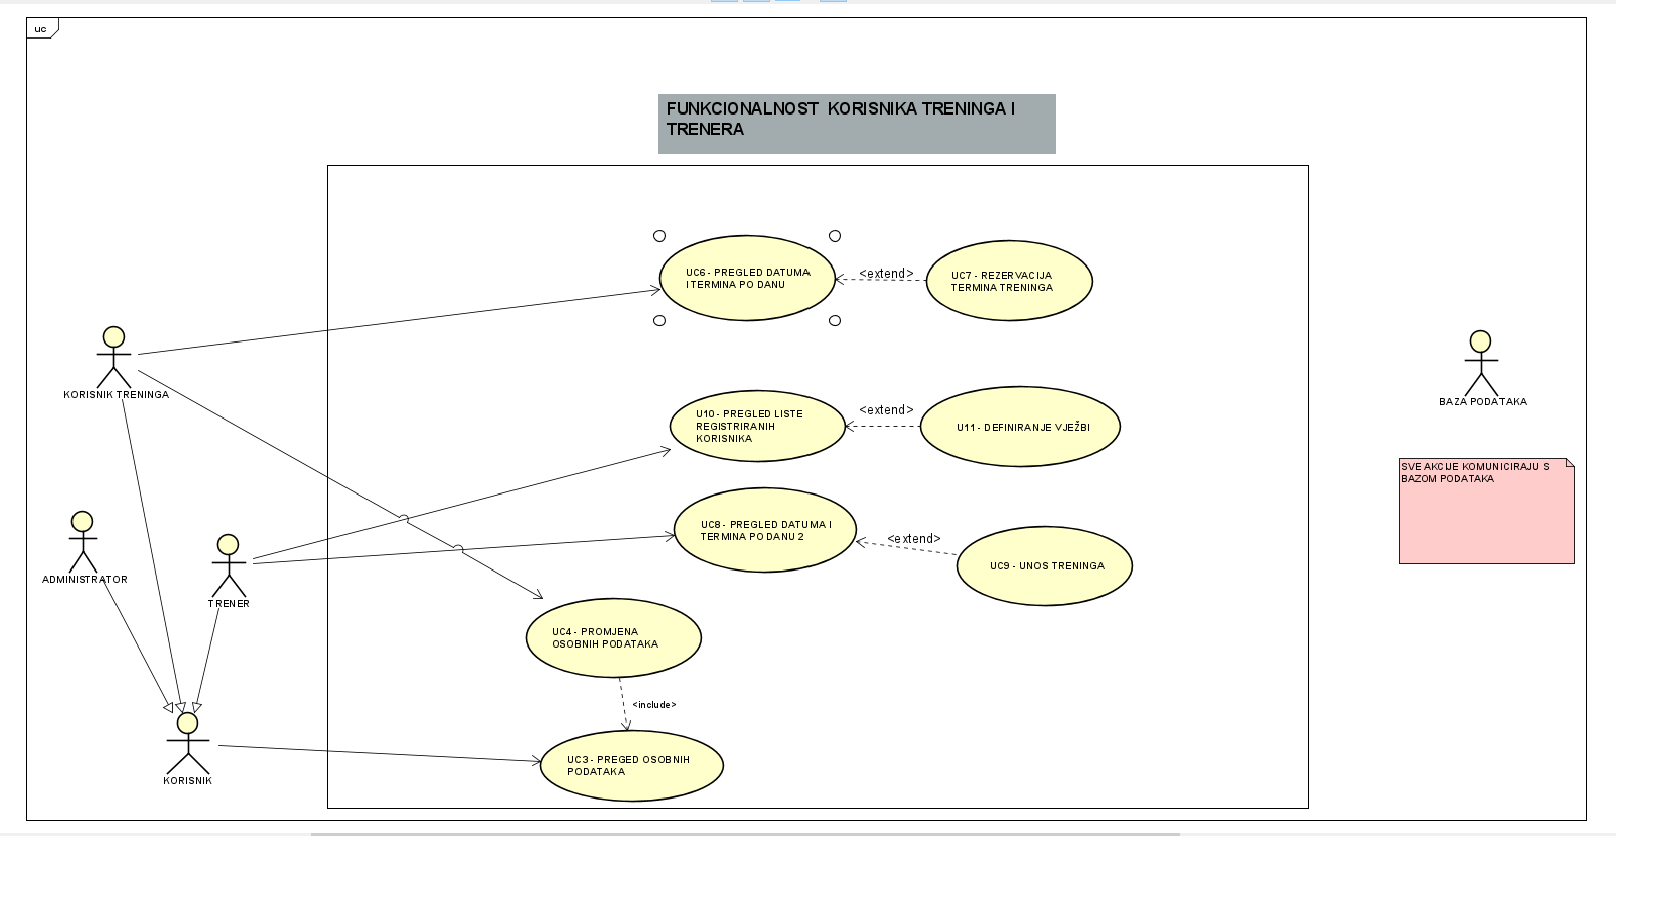
\includegraphics[scale=0.5]{dijagrami/drugidijagramou.png} %veličina slike u odnosu na originalnu datoteku i pozicija slike
			     		\centering
			     		\caption{"Dijagram funkcionalnosti korisnika treninga i trenera"}
			     		\label{fig:ou2}
			     	\end{figure}
		     	
		     	\begin{figure}[H]
		     		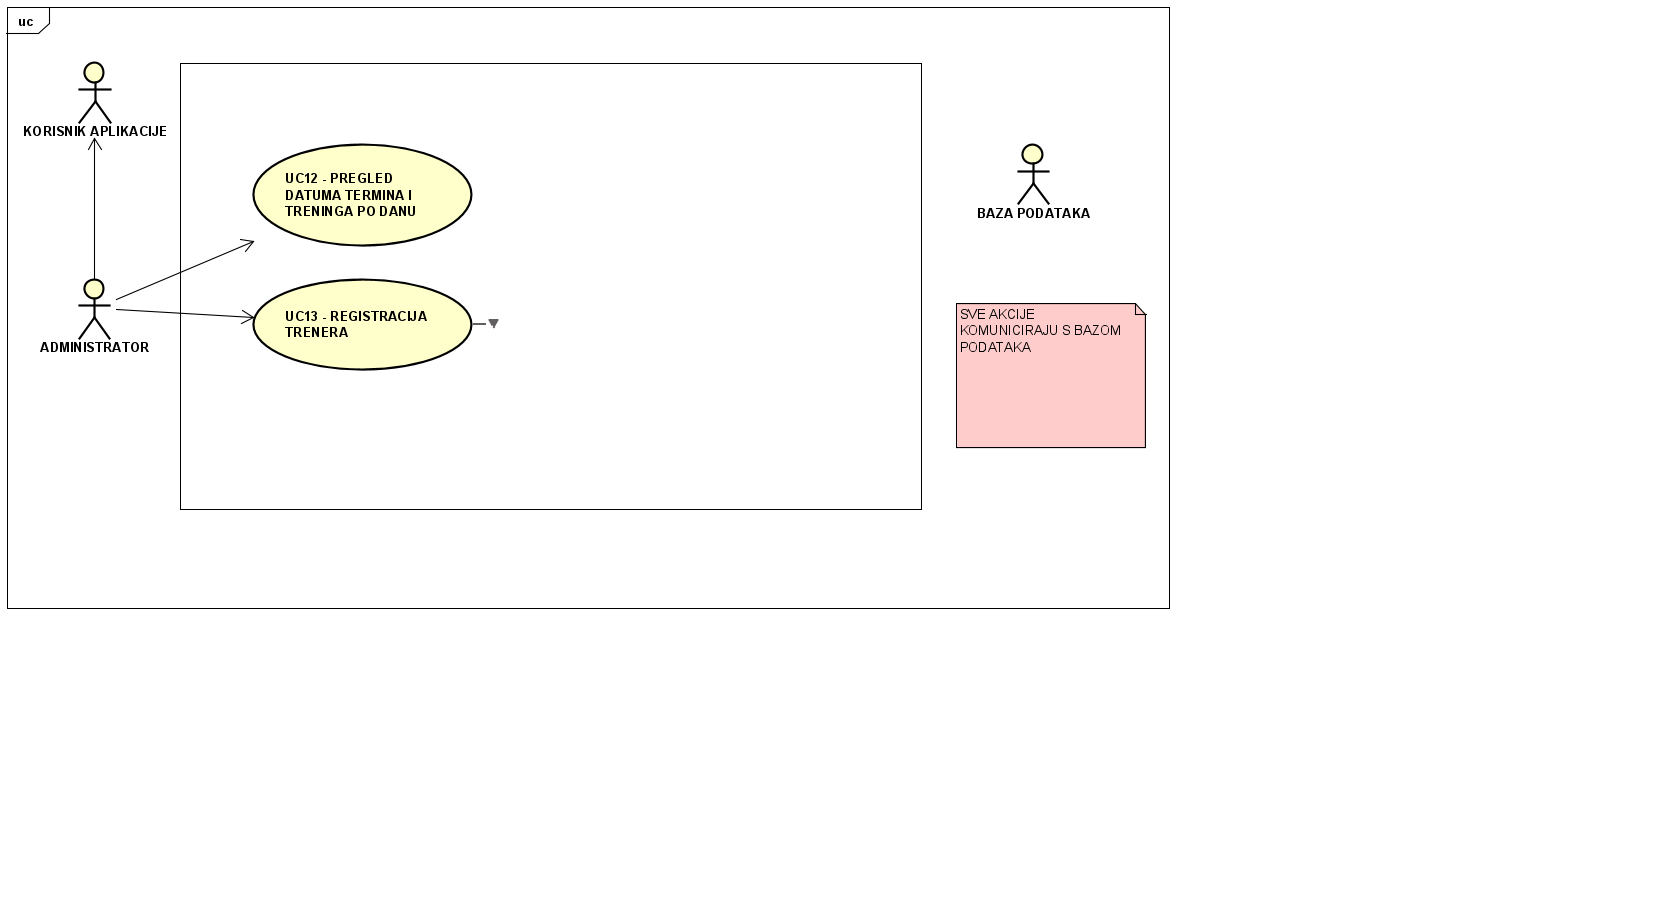
\includegraphics[scale=0.5]{dijagrami/trecidijagramou.png} %veličina slike u odnosu na originalnu datoteku i pozicija slike
		     		\centering
		     		\caption{"Dijagram funckionalnosti korisnika aplikacije i administratora"}
		     		\label{fig:ou3}
		     	\end{figure}
					
			\subsection{Sekvencijski dijagrami}
				
				

				\textbf{\textit{Obrazac uporabe UC1 - Registracija}}\\
	
				{Klijent šalje zahtjev za stranicu registracije kako bih se mogao registrirati. Poslužitelj dohvaća stranicu za registraciju te ju prikazuje. Zatim klijent ispunjava formu za registraciju te ju šalje poslužitelju. Poslužitelj provjerava ispravnost podataka te ukoliko su ispravni zapisuje podatke u bazu podataka. Nakon uspješne registracije poslužitelj klijentu prikazuje stranicu s osobnim podacima.
					
				
				\begin{figure}[H]
					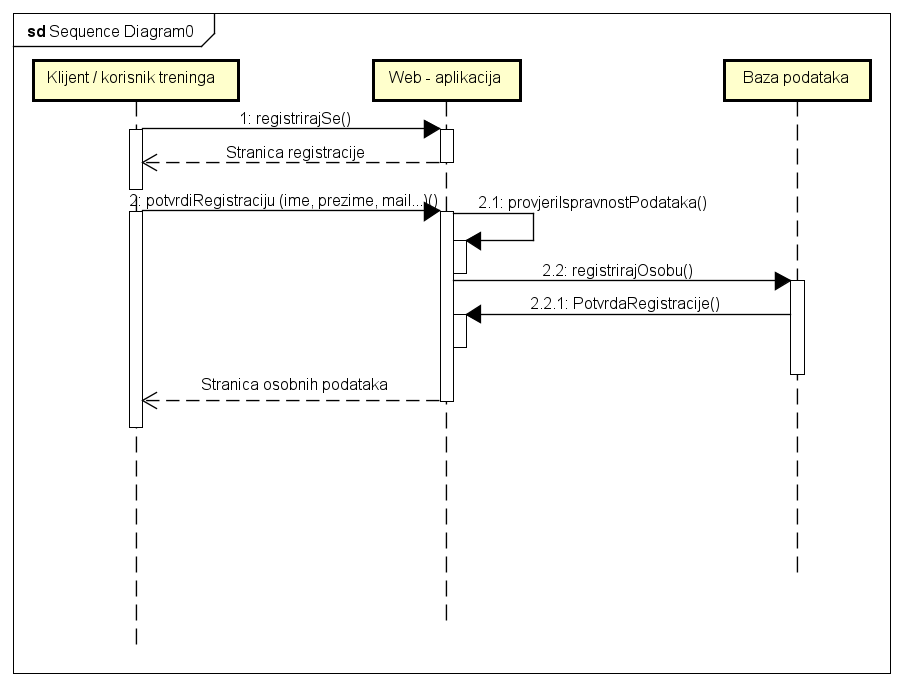
\includegraphics[scale=0.6]{dijagrami/sekvencijskiVukelic.png} %veličina slike u odnosu na originalnu datoteku i pozicija slike
					\centering
					\caption{"Registracija"}
					\label{fig:sekvencijski1}
				\end{figure}
			
				\eject
				
				\textbf{\textit{Obrazac uporabe UC7 - Rezervacija termina treninga}}\\
				
			
				{Klijent šale zahtjev za prikaz stranice za prijavu. Poslužitelj vraća stranicu za prijavu te klijent nastavlja s prijavom unoseći svoje podatke(username i password). Nakon unosa podataka poslužitelj provjerava ispravnost podataka sa bazom podataka te ukoliko je uspješno poslužitelj klijentu prikazuje stranicu kalendara. Zatim klijent bira željene termine te poslužitelj provjerava u bazi podataka ima li klijent dovoljno sati u vlastitom fondu. Ukoliko nema prikazuje se alert poruka u suprotnom poslužitelj sprema odabrane termine klijenta u bazu podataka te umanjuje preostali fond sati klijenta. Nakon obavljenih operacija poslužitelj klijentu prikazuje tipku "odustani" ukoliko klijent želi odustati od rezerviranih termina.}
				
				
				\begin{figure}[H]
					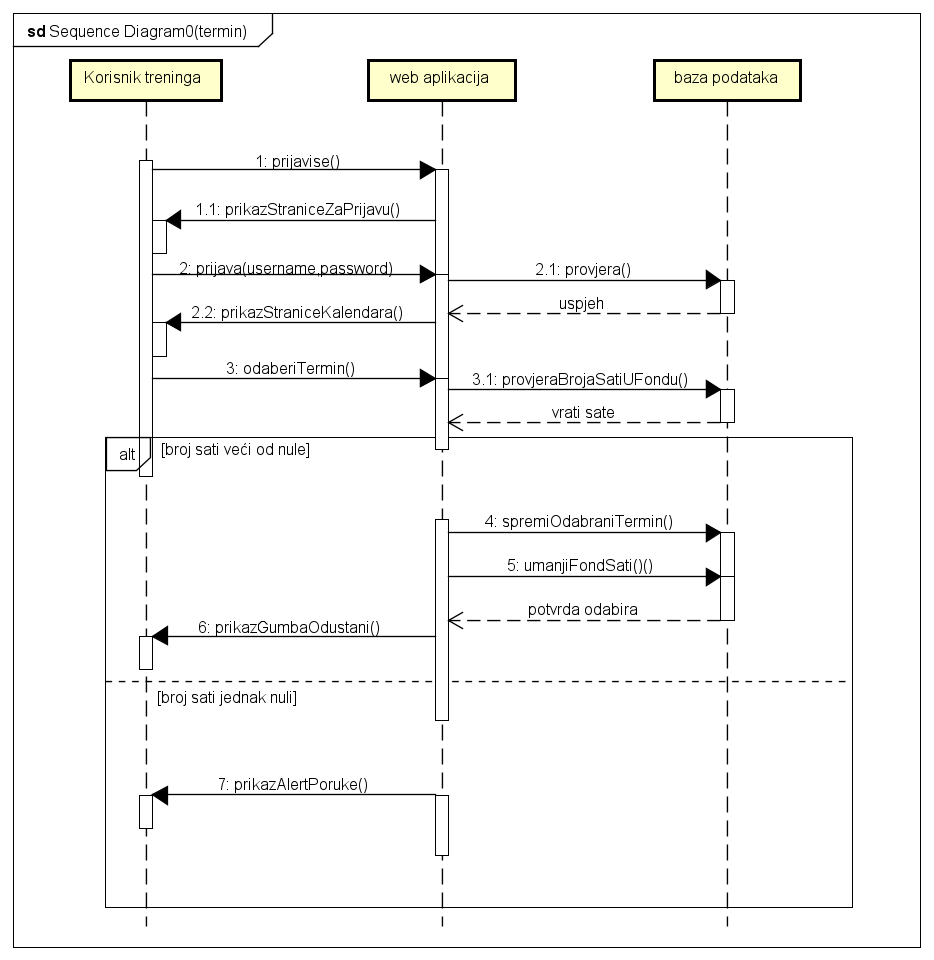
\includegraphics[scale=0.6]{dijagrami/UC7fixedsequental.png} %veličina slike u odnosu na originalnu datoteku i pozicija slike
					\centering
					\caption{"Rezervacija termina treninga"}
					\label{fig:sekvencijski2}
				\end{figure}
				
				\eject
				
				\textbf{\textit{Obrazac uporabe UC9 - Unos treninga}}\\
				
				
				{Klijent u ovom slučaju trener šalje zahtjev za prikaz stranice kalendara. Poslužitelj vraća stranicu kalendara te trener nastavlja s unosom termina treninga birajući na kalendaru u kojem terminu želi da se trening odvija. Nakon odabira termina poslužitelj sprema odabrani termin u bazu podataka zajedno s vježbama koje će se obavljati tokom treninga. Nakon spremanja u bazu podataka poslužitelj mjenja boju termina kako bih znali da je termin popunjen. }
				
				
				\begin{figure}[H]
					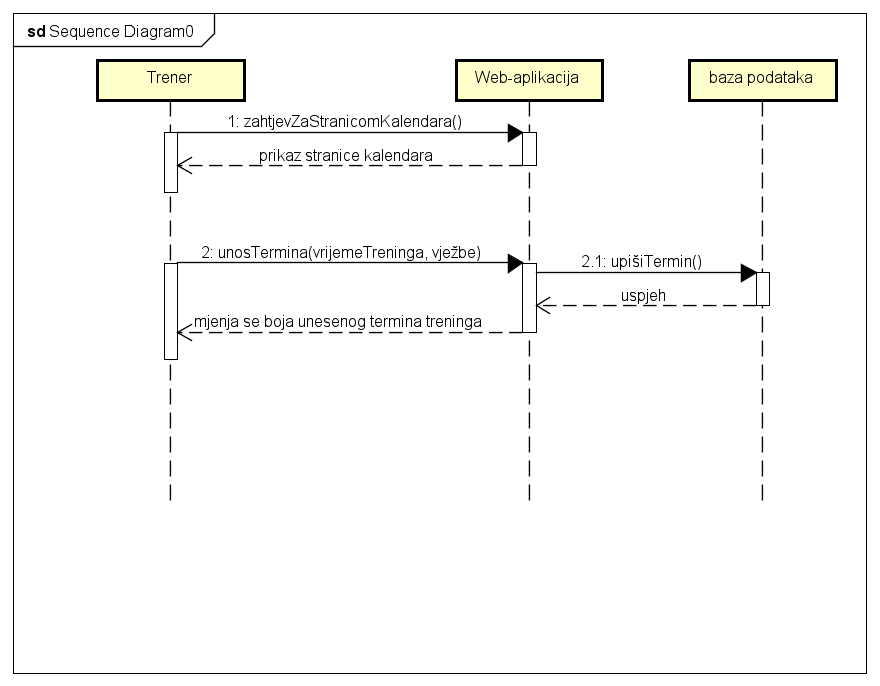
\includegraphics[scale=0.6]{dijagrami/UC9sekvencijski.png} %veličina slike u odnosu na originalnu datoteku i pozicija slike
					\centering
					\caption{"Unos treninga"}
					\label{fig:sekvencijski3}
				\end{figure}
				
				\eject
				
				\textbf{\textit{Obrazac uporabe UC14 - Odjava}}\\
				
				
				{Klijent zatraži od poslužitelja stranicu osobnih podataka. Poslužitelj vraća klijentu stranicu poslužitelja te zatim klijent klikne gumb "logout". Poslužitelj zatim odjavljenom korisniku prikazuje početnu stranicu web aplikacije.}
				
				
				\begin{figure}[H]
					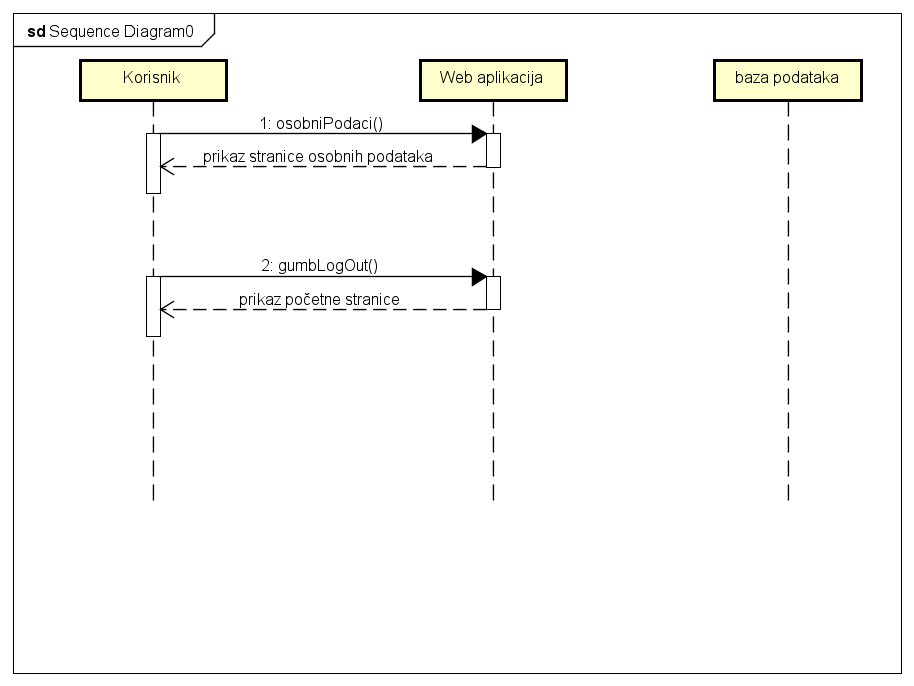
\includegraphics[scale=0.6]{dijagrami/UC14.png} %veličina slike u odnosu na originalnu datoteku i pozicija slike
					\centering
					\caption{"Odjava"}
					\label{fig:sekvencijski4}
				\end{figure}
				
				\eject

		\section{Ostali zahtjevi}
			 
			 \begin{packed_item}
			 	\item { Aplikacija treba biti izvedena kao web aplikacija kojoj će korisnici pristupati uz pomoć korisničkog imena i lozinke}
			 	\item {Aplikacija treba biti jednostavna za korištenje, a sučelje pregledno i intuitivno}
			 	\item {Aplikacija treba biti prilagođena za rad na različitim uređajima (mobilni uređaj, tablet, PC)}
			 	\item {Aplikacija mora osigurati sigurnost baze podataka i otpornost na vanjske prijetnje}
			 	\item {Aplikacija mora omogućiti rad više korisnika istovremeno}
			 	\item {Korisničko sučelje treba podržavati englesku abecedu pri unosu i prikazu sadržaja}
			 \end{packed_item}
			 
			 
			 
	